\section*{CHƯƠNG 1: GIỚI THIỆU}
\addcontentsline{toc}{section}{\numberline {} CHƯƠNG 1: GIỚI THIỆU}
\setcounter{section}{1}
\subsection{TỔNG QUAN}
\subsubsection{Đặt vấn đề}
IoT (Internet of things) được dịch sang tiếng Việt với nhiều tên gọi khác nhau như Internet Vạn Vật, Mạng lưới thiết bị kết nối Internet, Mạng lưới vạn vật kết nối Internet,… Trong đó, thuật ngữ được sử dụng phổ biến nhất là Internet Vạn Vật.\\
\indent IoT là một liên mạng với sự tham gia của nhiều thành phần. Trong đó, các thiết bị, phương tiện sẽ được bổ sung và tích hợp thêm các bộ phận điện tử, phần mềm cũng như các loại cảm biến giúp chúng vừa có thể thu thập dữ liệu, vừa có thể kết nối qua mạng máy tính để truyền và chia sẻ các dữ liệu đó. Hệ thống các thiết bị, phương tiện thông minh này sẽ tạo nên một cơ sở hạ tầng đáp ứng nhu cầu phát triển của xã hội thông tin \cite{bor2016lora}.\\
\indent IoT là công nghệ đóng vai trò quan trọng và bắt đầu tác động đến nhiều lĩnh vực và ngành công nghiệp, từ sản xuất, y tế, truyền thông, năng lượng cho đến ngành nông nghiệp. IoT bao gồm cơ sở hạ tầng truyền thông cơ bản được sử dụng để kết nối các đối tượng thông minh từ cảm biến, phương tiện, thiết bị di động đến việc thu thập dữ liệu từ xa dựa trên phân tích thông minh, giao tiếp người dùng và cách mạng hóa ngành nông nghiệp.\\
\indent Bằng cách triển khai các công nghệ cảm biến và IoT trong thực tiễn nông nghiệp đã làm thay đổi mọi khía cạnh của phương pháp canh tác truyền thống. IoT giúp cải thiện các giải pháp về canh tác truyền thống như ứng phó với hạn hán, tối ưu hóa năng suất, tính phù hợp đất đai, tưới tiêu và kiểm soát dịch hại.\\
\indent MQTT (Đầy đủ là Message Queuing Telemetry Transport) là một giao thức gửi tín hiệu dạng publish/subscribe. Chúng được sử dụng cho các thiết bị Internet of Things – IoT. Tín hiệu truyền đi với băng thông thấp, có độ tin cậy cao và khả năng sử dụng được trong mạng lưới thiếu ổn định. Bởi vì giao thức MQTT này sử dụng băng thông khá thấp trong môi trường có độ trễ cao nên nó là một giao thức lý tưởng cho các ứng dụng M2M (Machine to Machine).\\
\indent Công nghệ LoRa , được phát triển bởi Semtech , là một giao thức không dây mới được thiết kế để truyền thông tầm xa, năng lượng thấp. Giao thức cung cấp loại khả năng liên lạc mà các thiết bị thông minh cần có, và Liên minh LoRa đang hoạt động để đảm bảo khả năng tương tác giữa nhiều mạng trên toàn quốc.\\
\indent Một phần của phổ LoRa sử dụng thể hiện ít nhiễu điện từ, do đó tín hiệu có thể kéo dài một khoảng cách xa, thậm chí đi qua các tòa nhà, với rất ít năng lượng. Điều này phù hợp với các thiết bị IoT với dung lượng pin hạn chế. Điều đó cũng có nghĩa là các tinh thể chi phí thấp hơn có thể được sử dụng, do đó, việc xây dựng LoRa thành các thiết bị rẻ hơn.\\
\indent Mỗi gateway LoRa có thể xử lý hàng triệu node. Điều đó, cộng với thực tế là các tín hiệu có thể kéo dài khoảng cách đáng kể, có nghĩa là cần ít cơ sở hạ tầng mạng hơn, do đó làm cho việc xây dựng mạng LoRa rẻ hơn. Các mạng LoRa có thể được đặt cùng với các thiết bị liên lạc khác, như các tháp điện thoại di động, làm giảm đáng kể các hạn chế xây dựng.\\
\indent Các tính năng khác của LoRa cũng khiến nó trở nên lý tưởng cho IoT. LoRa sử dụng thuật toán tốc độ dữ liệu thích ứng để giúp tối đa hóa tuổi thọ pin và dung lượng mạng của thiết bị. Các giao thức của nó bao gồm nhiều lớp mã hóa, ở cấp độ mạng, ứng dụng và thiết bị, cho phép liên lạc an toàn. Tính hai chiều của giao thức hỗ trợ các thông điệp quảng bá, cho phép chức năng cập nhật phần mềm.\\
\indent Sự phát triển của Internet of Things bị giới hạn bởi dung lượng của mạng, bởi khả năng hoạt động của thiết bị mà không cần thay pin và bởi khả năng mã hóa truyền dẫn bí mật. Các tính năng được tích hợp trong LoRa cung cấp tất cả các khả năng này và sẽ cho phép sự phát triển rộng rãi của IoT.\\
\indent Với công nghệ Lora , chúng ta có thể truyền dữ liệu với khoảng cách lên hàng km mà không cần các mạch khuếch đại công suất; từ đó giúp tiết kiệm năng lượng tiêu thụ khi truyền/nhận dữ liệu. Do đó, LoRa có thể được áp dụng rộng rãi trong các ứng dụng thu thập dữ liệu như sensor network trong đó các sensor node có thể gửi giá trị đo đạc về trung tâm cách xa hàng km và có thể hoạt động với battery trong thời gian dài trước khi cần thay pin.\\
\\

\indent Nhận thấy những ưu điểm của Lora, giao thức MQTT và những ứng dụng vô cùng thực tế của IoT trong nông nghiệp. Chính vì vậy mục tiêu của đề tài tạo ra mạng kết nối với các thiết bị dùng để điều khiển, các cảm biến thu thập dữ liệu, vẽ đồ thị trạng thái dựa trên dữ liệu thu thập được từ cảm biến thông qua mạng LoRa và giao thức MQTT.
\subsubsection{Tình hình nghiên cứu trong nước}
Qua tìm hiểu về tình hình nghiên cứu, trong nước rất ít dự án ứng dụng công nghệ LoRa đưa vào thực tế. Tuy nhiên cũng có rất nhiều dự án, công trình đã và đang được nghiên cứu:
\begin{itemize}
	\item Lê Đình Vương, MSSV 41204661, đề tài luận văn "Thu thập và quản lí dữ liệu thông qua mạng LoRa", Đại học Bách Khoa TP.HCM, tháng 6 năm 2017.
	\item Nguyễn Quốc Anh, MSSV 21300108, đề tài luận văn "Thiết kế hệ thống đo lường chất lượng hồ nuôi tôm sử dụng công nghệ LoRa", Đại học Bách Khoa TP.HCM, tháng 5 năm 2018.
\end{itemize}
\subsubsection{Tình hình nghiên cứu ngoài nước}
Hiện nay có nhiều cá nhân, công ty nghiên cứu phát hành sản phẩm LoRa mộthay nhiều kênh truyền dựa trên chipset của Semtech. Các công trình nghiên cứu:
\begin{itemize}
	\item Đề tài “A DIY low-cost LoRa gateway” của Giáo sư Phạm Công Đức, trường đại học Paul, Pháp sử dụng chip SX1276 của Semtech với Gateway một kênh truyền.
	\item Module LoRaWan IXM-LPWA-800-16-K9 của Cisco cho các ứng dụng cần công suất thấp, diện tích phủ rộng lớn như tracking vật thể, đo nước hay khí.
\end{itemize}
\subsection{NHIỆM VỤ THỰC TẬP}
\subsubsection{Mục tiêu đề tài}
Thực hiện truyền dữ liệu nhiệt độ, độ ẩm từ End-node thông qua LoRa về Gateway, Gateway chuyển tiếp dữ liệu thông qua giao thức MQTT về App điện thoại thông minh.\\
\indent Truyền lệnh điều khiển bật/tắt đèn từ App điện thoại thông minh về Gateway thông qua giao thức MQTT, Gateway chuyển tiếp đến End-node thực hiện lệnh thông qua LoRa
\subsubsection{Yêu cầu đề tài}
\begin{itemize}
	\item \textbf{Nội dung 1:} Tìm hiểu module RF UART Lora E32-TTL-100 SX1278 SEMTECH
	\item \textbf{Nội dung 2:} Tìm hiểu MQTT và LoRa
	\item \textbf{Nội dung 3:} Xây dựng App Android
\end{itemize}
\subsubsection{Kế hoạch thực hiện}
\begin{figure}[H]
	\centering
	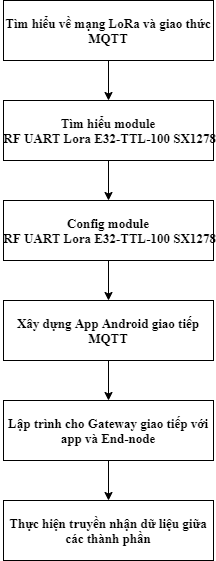
\includegraphics[scale=.5]{Chapter 1/image chapter 1/kehoachthuchien.png}
	\caption[Kế hoạch thực hiện]{Kế hoạch thực hiện}
	\label{hinh11}
\end{figure}
